\documentclass{article}
\usepackage{color}
\usepackage{graphicx}
\usepackage{setspace}
\usepackage{hyperref}
\usepackage{geometry}
\usepackage{amsmath}
\usepackage{enumitem,amssymb}
\usepackage{pifont}
\definecolor{darkgreen}{rgb}{0.0, 0.5, 0.0}
\geometry{left = 1.25in, right=1.25in} % New Stuff Learned!
\newcommand{\cmark}{\ding{51}}
\newcommand{\xmark}{\ding{55}}
\newcommand{\done}{\rlap{$\square$}{\raisebox{2pt}{\large\hspace{1pt}\cmark}}
\hspace{-2.5pt}}
\newcommand{\wontfix}{\rlap{$\square$}{\large\hspace{1pt}\xmark}}
\newlist{todolist}{itemize}{2}
\setlist[todolist]{label=$\square$}
\doublespacing
\begin{document}
\begin{titlepage}

\title{\textbf{CHE374 Week 1}}
\author{\textit{Sanzhe Feng}}
\date{\textit{\today}}
\maketitle
\end{titlepage}
\setlength{\parindent}{0pt}

\section*{Motivation of Unsupervised Learning}
Usually, it is hard and expensive to collect labeled data required for supervised learning.

- Generative modeling

- Self-supervised learning

- Compression

In this course, we will be looking at three applications of unsupervised learning:

- Clustering: recommendation/search results, marktet segmentation, social network analysis

- Dimensionality reduction: get rid of redundancy

- Data visualization

\section*{Clustering with the k-means algorithm}

k-mean algorithm is used to find the clusters of data.

First, randomly select two cluster centroids. Compute the distance between the each data to the centroids, then we assign each data point to the centroid that is closest to it.

Then we update the location of the centroids by computing the mean of all the points that have been assigned to each cluster. 

Reset all data points to be unassigned. Repeat the distance calculation and the relocation of centroids. 


\subsection*{k-mean algorithm}
- input: k number of clusters; training set $\{x^{1}...x^{n}\}$

- random initialization: k cluser centroids $\mu_1...\mu_k$

- Repeat: 
    for i in 1 to m

    \hspace{1.1cm}$c^{(i)}$ = index of cluster centroid closest to $x^i$

    for k in 1 to k

    \hspace{1.1cm}$\mu_k$ = mean of points assigned to cluseter k


\section*{Distortion in the k-means algorithm}

\subsection*{Optimization objective }
Cost function: $J(c^1, ... , c^m, \mu_1, ..., \mu_u) = \frac{1}{m}\sum ||x^i -\mu_c||^2$

2 steps of k-mean algorithms:

1. Cluster assignment step: minimizing cost function wrt to c while fixing $\mu$

2. Move centroids step: minimizing cost function wrt $\mu$ while fixing c

\subsection*{Initialization}
How to pick the value of K:

                            
Strategy is to pick random points as K in the input domain or K training sets as the K initial cluster centroids. 

\subsection*{Local Optima}
Problem that caused by initialization. 

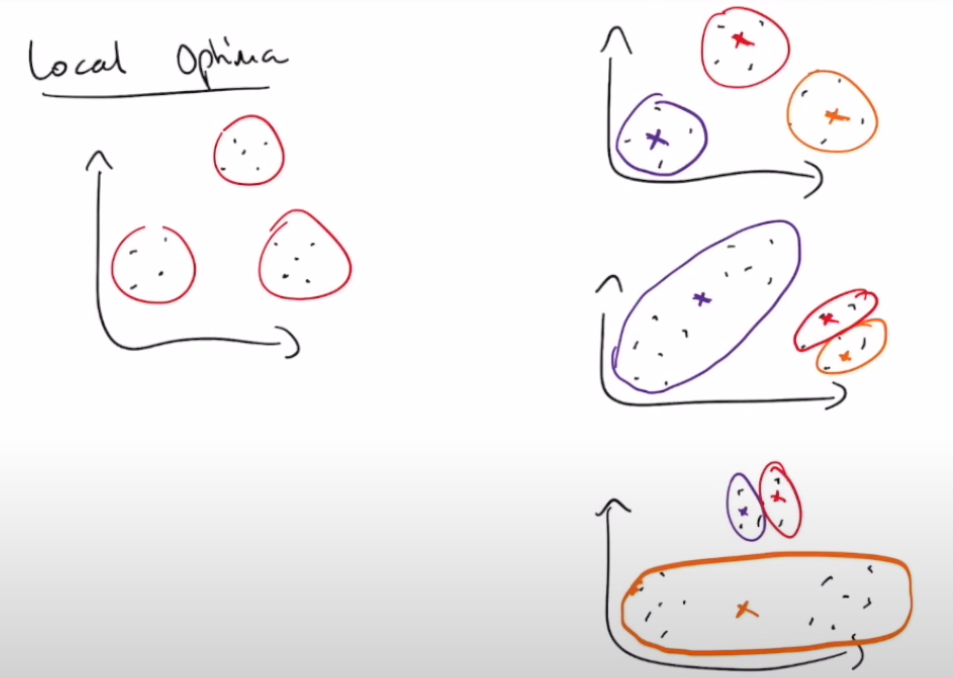
\includegraphics[width=0.7\linewidth]{W2V3.png}

\end{document}